\documentclass{article}
\usepackage{natbib}
\usepackage{graphicx}
\usepackage{csquotes}
\usepackage{hyperref}
\usepackage{booktabs}
\usepackage{multirow}
\usepackage[table]{xcolor} 
\usepackage{graphicx}

%---------------------------------- NATBIB ----------------------------------%
\makeatletter
% natbib: only make year a hyperref, not author
\let\oldciteauthor\citeauthor

\def\citeauthor#1{{\NoHyper\oldciteauthor{#1}}}

% Patch case where name and year are separated by aysep
\patchcmd{\NAT@citex}
  {\@citea\NAT@hyper@{%
     \NAT@nmfmt{\NAT@nm}%
     \hyper@natlinkbreak{\NAT@aysep\NAT@spacechar}{\@citeb\@extra@b@citeb}%
     \NAT@date}}
  {\@citea\NAT@nmfmt{\NAT@nm}%
   \NAT@aysep\NAT@spacechar\NAT@hyper@{\NAT@date}}{}{}

% Patch case where name and year are separated by opening bracket
\patchcmd{\NAT@citex}
  {\@citea\NAT@hyper@{%
     \NAT@nmfmt{\NAT@nm}%
     \hyper@natlinkbreak{\NAT@spacechar\NAT@@open\if*#1*\else#1\NAT@spacechar\fi}%
       {\@citeb\@extra@b@citeb}%
     \NAT@date}}
  {\@citea\NAT@nmfmt{\NAT@nm}%
   \NAT@spacechar\NAT@@open\if*#1*\else#1\NAT@spacechar\fi\NAT@hyper@{\NAT@date}}
  {}{}
  
\makeatother
%-------------------------------------------------------------------------------%


%----------------------------------- HREF ------------------------------------%
% define href colors
\hypersetup{
    colorlinks=true,
    linkcolor=blue,
    filecolor=blue,      
    urlcolor=blue,
    citecolor=blue
}
\urlstyle{same}
%-------------------------------------------------------------------------------%


\begin{document}
\graphicspath{ {../../../output/03-results/plots/} }

\section{What Has to be Mentioned Before}
\label{sec:before}

\section{Data}

The data for this study comprises two distinct corpora: a corpus with legal documents and a baseline corpus with comments from Reddit, the world's largest online-forum. The legal corpus contains court opinions from Court of Appeals for 1st to 11th circuit, based on open data provided by the \citet{FreeLawProject2020}. For the baseline corpus, we gathered data using the API for the Pushshift Reddit Data Set provided by \citet{Baumgartner2020}. 

In our case, the corpus generation is an iterative process. We start off with a list of target adjectives we specified without information about the corpora. This initial list, $L_1$, includes 2x5 adjectives often discussed by the TC-literature and we deem rather uncontroversial examples of epistemic concepts, thick and thin concepts as well as legal concepts. However, some of these adjectives are rarely used in the legal context, while others may occur frequently, yet are most often part of legal phrases, which indicate a different semantic embedding. In order to avoid any sort of selection bias and exclude adjectives with predominantly phrasal use, we inductively select a second battery of adjectives. This inductive approach is based on an analysis of part of speech (PoS)-sequences in the legal corpus. PoS-tagging is an unsupervised method to annotate the syntactic structure of text data. For each of the subcorpora (1st to 11th Court of Appeals), we first draw a random sample of 2000 documents which are subsequently PoS-tagged using UDPipe \citep{Straka2017, Straka2020}. Based on these PoS-tags, we isolate all syntactic structures of the form $(M)*A(,)*C(M)*A$ (M = modifier, A = adjective, C = conjunction, (...) = optional part). The conjuncts are then pooled across all subcorpora and only AND-conjunctions are retained. Finally, all adjectives %$A_i...A_n$ 
are ranked according to frequency as well lexical diversity in regards to the conjoined adjectives. We use Yule's \textit{K} \citep{Yule1944, Tweedie1998} as a measure for lexical diversity.  %In addition, we map them on a dissociation dimension, which gives a measure of how exclusive the set of conjoined adjectives is for a specific $A_i$.
Based on this ranking, we manually select adjectives that match our concept classes and add antonyms to form list $L_2$. In a third step, we combine $L_1$ and $L_2$, and use them to retrieve documents containing suitable target structures both from the legal corpus and via the Pushshift API. The combined list is shown in \ref{tab:l3} in the \ref{sec:appendix}. 

The full legal corpus has XXX entries, the baseline corpus XXX. In order to keep the computational resources low while keeping a high enough $n$, we reduce the legal subcorpora each randomly by -40\%, resulting in XXX legal documents overall. Both corpora are subsequently cleaned, PoS-tagged, lemmatized and the conjoined adjectives are annotated with sentiment values from the SentiWords dictionary based on SENTIWORDNET \citep{Esuli2006, Baccianella2010, Guerini2013, Gatti2016}.

\section{Method}

In the following, we will discuss the methods used in our two studies.

\subsection{Study 1}



\subsection{Study 2}

In the second study, we focus on the legal corpus only. In order to be able to compare the results of the evaluative concepts classes to a baseline, we added corpus entries for the following descriptive target adjectives: . Instead of comparing context effects (Study 1), we want to inquire whether the concept classes cluster differently within the legal context. We use a combination of K-Means Clustering and Principal Component Analysis (PCA), which is informed by the sentiment values of the conjoined adjectives and a measure for lexical diversity of the target adjective, i.e. Yule's \textit{K} \citep{Yule1944, Tweedie1998}. The cluster analysis further includes information based on the vector space of the corpus, which is created using the \textit{Semantic Vectors} package \citep{Widdows2008, Widdows2010, Widdows2016}. For every pair of target adjective and conjoined adjective, we compute the cosine similarities. Cosine similarities are essentially high dimensional representations of co-occurence measures, and inform the cluster analysis about the semantic similarity of the conjuncts by taking the whole corpus into account. In the final ANOVA model, the cosine similarities are added as weights for the sentiment values of the conjoined adjectives.

\section{Results}

\subsection{Descriptive Statistics}

\begin{table}[ht]
\centering
\rowcolors{5}{gray!25}{white}
\begin{tabular}{rlrrrrrrrr}
  & & \multicolumn{3}{c}{Sentiment Quantiles} & & \multicolumn{3}{c}{Lex. Diversity}\\
   \cmidrule{3-5} \cmidrule{7-9}
  Class & Polarity & 25\% & 50\% & 75\% & Avg. &  TTR & CTTR & K\\
  \bottomrule
Descriptive & neutral & -0.18 & 0.00 & 0.22 & 0.02 & 0.15 & 6.17 & 168.36 \\ 
  Epistemic & negative & -0.44 & -0.33 & -0.10 & -0.26 & 0.16 & 6.09 & 124.78 \\ 
  Epistemic & positive & 0.04 & 0.14 & 0.30 & 0.17 & 0.05 & 3.68 & 342.11 \\ 
  Legal & negative & -0.40 & -0.29 & 0.00 & -0.19 & 0.13 & 4.69 & 249.80 \\ 
  Legal & positive & 0.07 & 0.22 & 0.22 & 0.17 & 0.04 & 2.93 & 1530.47 \\ 
  TC & negative & -0.44 & -0.35 & -0.20 & -0.30 & 0.11 & 4.81 & 507.77 \\ 
  TC & positive & 0.06 & 0.16 & 0.33 & 0.21 & 0.06 & 3.55 & 640.33 \\ 
   \hline
\end{tabular}
\caption{Summary Statistics Legal Corpus}
\end{table}

\begin{table}[ht]
\centering
\rowcolors{5}{gray!25}{white}
\begin{tabular}{rlrrrrrrrr}
  & & \multicolumn{3}{c}{Sentiment Quantiles} & & \multicolumn{3}{c}{Lex. Diversity}\\
   \cmidrule{3-5} \cmidrule{7-9}
  Class & Polarity & 25\% & 50\% & 75\% & Avg. &  TTR & CTTR & K\\
  \bottomrule
Epistemic & negative & -0.52 & -0.42 & -0.18 & -0.34 & 0.10 & 7.65 & 73.19 \\ 
  Epistemic & positive & 0.16 & 0.29 & 0.50 & 0.30 & 0.08 & 7.26 & 94.69 \\ 
  Legal & negative & -0.55 & -0.44 & -0.24 & -0.38 & 0.13 & 6.65 & 198.62 \\ 
  Legal & positive & 0.00 & 0.22 & 0.45 & 0.21 & 0.09 & 6.43 & 132.81 \\ 
  TC & negative & -0.55 & -0.45 & -0.29 & -0.39 & 0.09 & 6.93 & 80.10 \\ 
  TC & positive & 0.16 & 0.32 & 0.52 & 0.31 & 0.09 & 7.06 & 125.27 \\ 
   \hline
\end{tabular}
   \caption{Summary Statistics Baseline Corpus}
\end{table}

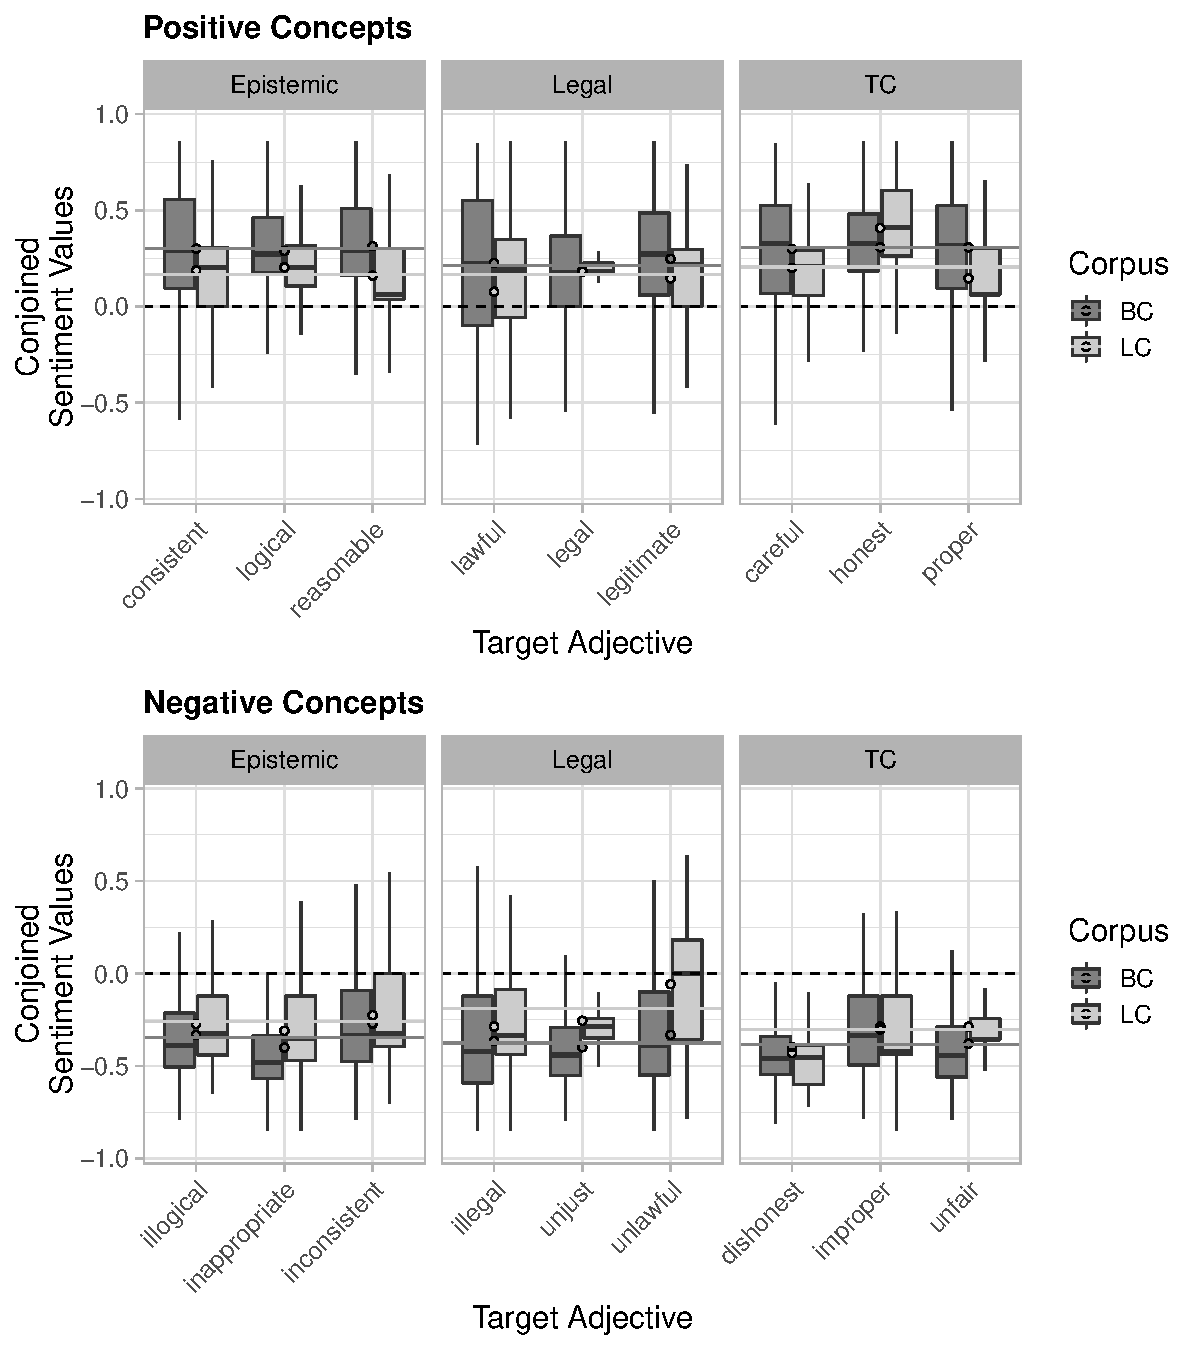
\includegraphics[width=\textwidth, keepaspectratio]{bc_lc_summary_stats_adj-distr}

\subsection{Study 1}


\subsection{Study 2}

\bibliographystyle{apalike}
\bibliography{legaltc-bib}

\section{Appendix}
\label{sec:appendix}



\end{document}